

\section{Method}
\subsection{Instruction-Driven Text Data Generation}
\label{sec3.1}
One of our main goals is to perform image-to-image tasks based on text instructions without losing the linguistic reasoning capabilities inherent in language models, rather than only generating accurate clinical reports. However, a common problem is that many medical datasets lack image-text pairs, which means we need to generate text data using available clinical information. Nevertheless, generated text data may contain misinformation or hallucinations. To minimize this risk, we build on previous work on generating medical text data with LLMs (shown in Figure \ref{fig2}). We guide the LLMs by providing instructions that include clinician-selected demonstrations from BioMed-VITAL \cite{cui2024biomedical}, along with a few image-text examples selected by clinicians. Recent research has shown that having several models work together can greatly reduce hallucinations \cite{du2023improving}, so we use multiple LLMs, including Gemini 1.5 \cite{team2023gemini}, LLaMA 3.2 \cite{grattafiori2024llama3herdmodels}, and GPT 4o-mini \cite{achiam2023gpt}, to reduce risk. The generated text is then reviewed and scored by GPT-4o. It is subsequently regenerated using this feedback, and the final text data are used as reports in the VQA set. The prompts used for this process and details are described in the Appendix.

\subsection{Stage I: Instruction Tuning}
LLMs are pretrained on large amounts of text data, making it very costly to retrain them from scratch for multimodal tasks. Therefore, we fine-tune a text-based LLM to learn visual information as well. Depending on the instruction, the response corresponding to an image can be generated as text, an image, or a segmentation mask by a single LLM. The image is also tokenized like text and fed to the LLM. Output image tokens are converted back to images by the VQ decoder. The pipeline is shown in Figure \ref{fig3}.

\vspace{3pt}
\noindent \textbf{Image Tokenization.}
To preserve the LLM's language ability during fine-tuning, we add image tokens to its existing vocabulary. For example, if the original LLM has an embedding table of size $\mathbb{R}^{K_\texttt{text}\times d_e}$ , where $d_e$ is the embedding dimension, the table is expanded to $\mathbb{R}^{(K_\texttt{text}+K_\texttt{img})\times d_e}$, where $K_\texttt{text}$ and $K_\texttt{img}$ represent the vocabulary size of text and image tokens, respectively. We use a VQ-GAN to tokenize images by compressing them into quantized latents. The VQ-GAN consists of an encoder $E$ and decoder $D$ as follows:
\begin{equation}
    E(\cdot):\mathbb{R}^{C\times H\times W} \rightarrow \{1,2,\ldots,K_\texttt{img}\}^{d_z}
\end{equation}
\begin{equation}
    D(\cdot):\{1,2,\ldots,K_\texttt{img}\}^{d_z} \rightarrow \mathbb{R}^{C\times H\times W}
\end{equation}
Using VQ-GAN, a tokenized latent $z$ of length $d_z$ is obtained with $z \in \{1,2, \\ \ldots,K_\texttt{img}\}$. The VQ-GAN is trained with the loss defined below:
\begin{equation} 
\mathcal{L}_{VQGAN} = \underbrace{||x - \hat{x}||^2}_{\text{Reconstruction}} + \underbrace{\mathcal{L}_{GAN}}_\text{GAN} + \underbrace{\mathcal{L}_{VQ}}_\text{Codebook}, 
\end{equation}
where $\mathcal{L}_{GAN}$ is the GAN loss \cite{isola2017image} and $\mathcal{L}_{VQ}$ is the quantization loss \cite{van2017neural,esser2021taming}. The VQ encoder and decoder are frozen during LLM training.

\vspace{3pt}
\noindent \textbf{Image to Text Generation.}
We train our model by applying instruction fine-tuning to an LLM pretrained on a large text corpus. This process only fine-tunes the LLM, where no structural changes are made to the model other than expanding the token embedding table. In this task, tokenized images are fed directly into the LLM so that the model learns visual information besides its language abilities. The model is then instructed to generate a report corresponding to the given image. The input image tokens are fed into the LLM along with the \texttt{<input>} token and the model produces a response corresponding to the instruction. The instructions for fine-tuning are provided in the Appendix. An example of text generation is shown below.

\vspace{6pt}
\begin{adjustbox}{scale=0.73}
\begin{minipage}{1.35\linewidth}
\begin{Verbatim}[frame=single, numbersep=5pt,
                 commandchars=\\\{\}]
\textbf{Instruction}: Generate free-text radiology reports for the provided brain MR images.
\textbf{Input}: \texttt{<input>} \texttt{<VQ172 VQ281 ... VQ511 VQ172>}
\textbf{Response}: The axial brain scan, captured using the T1-weighted modality, presents a ...
\end{Verbatim}
\end{minipage}
\end{adjustbox}
\vspace{3pt}

\vspace{3pt}
\noindent \textbf{Image to Image Translation.}
This task aims to generate a target modality or segmentation mask that matches the given instruction by processing image tokens. The input image tokens are provided with an \texttt{<input>} token and the output image tokens are produced with an \texttt{<output>} token. Since the LLM produces image tokens in the same way it generates text tokens, no extra module is required. For the segmentation task, the \texttt{<seg>} token is used instead of the \texttt{<output>} token. An example of image translation task is shown below.

\vspace{6pt}
\begin{adjustbox}{scale=0.73}
\begin{minipage}{1.35\linewidth}
\begin{Verbatim}[frame=single, numbersep=5pt,
                 commandchars=\\\{\}]
\textbf{Instruction}: Generate a brain MR image in T2  based on the T1 input.
\textbf{Input}: \texttt{<input>} \texttt{<VQ172 VQ092 ... VQ658 VQ172>}
\textbf{Response}: \texttt{<output>} \texttt{<VQ172 VQ335 ... VQ079 VQ172>}
\end{Verbatim}
\end{minipage}
\end{adjustbox}
\vspace{3pt}

\vspace{3pt}
\noindent \textbf{Training Objective.} 
The LLM is optimized using an autoregressive objective based on instruction-input pairs \cite{radford2018improving,brown2020language,liu2023visual}. For an image $\textbf{X}_\texttt{img}$ and an instruction $\textbf{X}_\texttt{instruct}$, our objective is to generate a response $\textbf{X}_\texttt{response}$ in an autoregressive manner. The loss is applied only to the tokens generated after the response according to the instruction tuning approach \cite{taori2023stanford,conover2023free}.
For a sequence of length $L$, the training loss is given by:
\begin{equation} 
\begin{split}
\mathcal{L}_\texttt{instruct} = -\log(p(\textbf{X}_\texttt{response}|\textbf{X}_\texttt{img},\textbf{X}_\texttt{instruct})) \\
= \sum_{i=1}^{L}p_\theta(\textbf{x}_i|\textbf{X}_\texttt{img}, \textbf{X}_\texttt{instruct}, \textbf{X}_{\texttt{response}, < i} ),
\end{split}
\end{equation}
where $\theta$ denotes the learnable parameters, and $\textbf{X}_{\texttt{response}, < i}$ denotes the response tokens before the current prediction token $\textbf{x}_i$.

\begin{figure} [t]
    \vspace{-6pt}
    \centering
    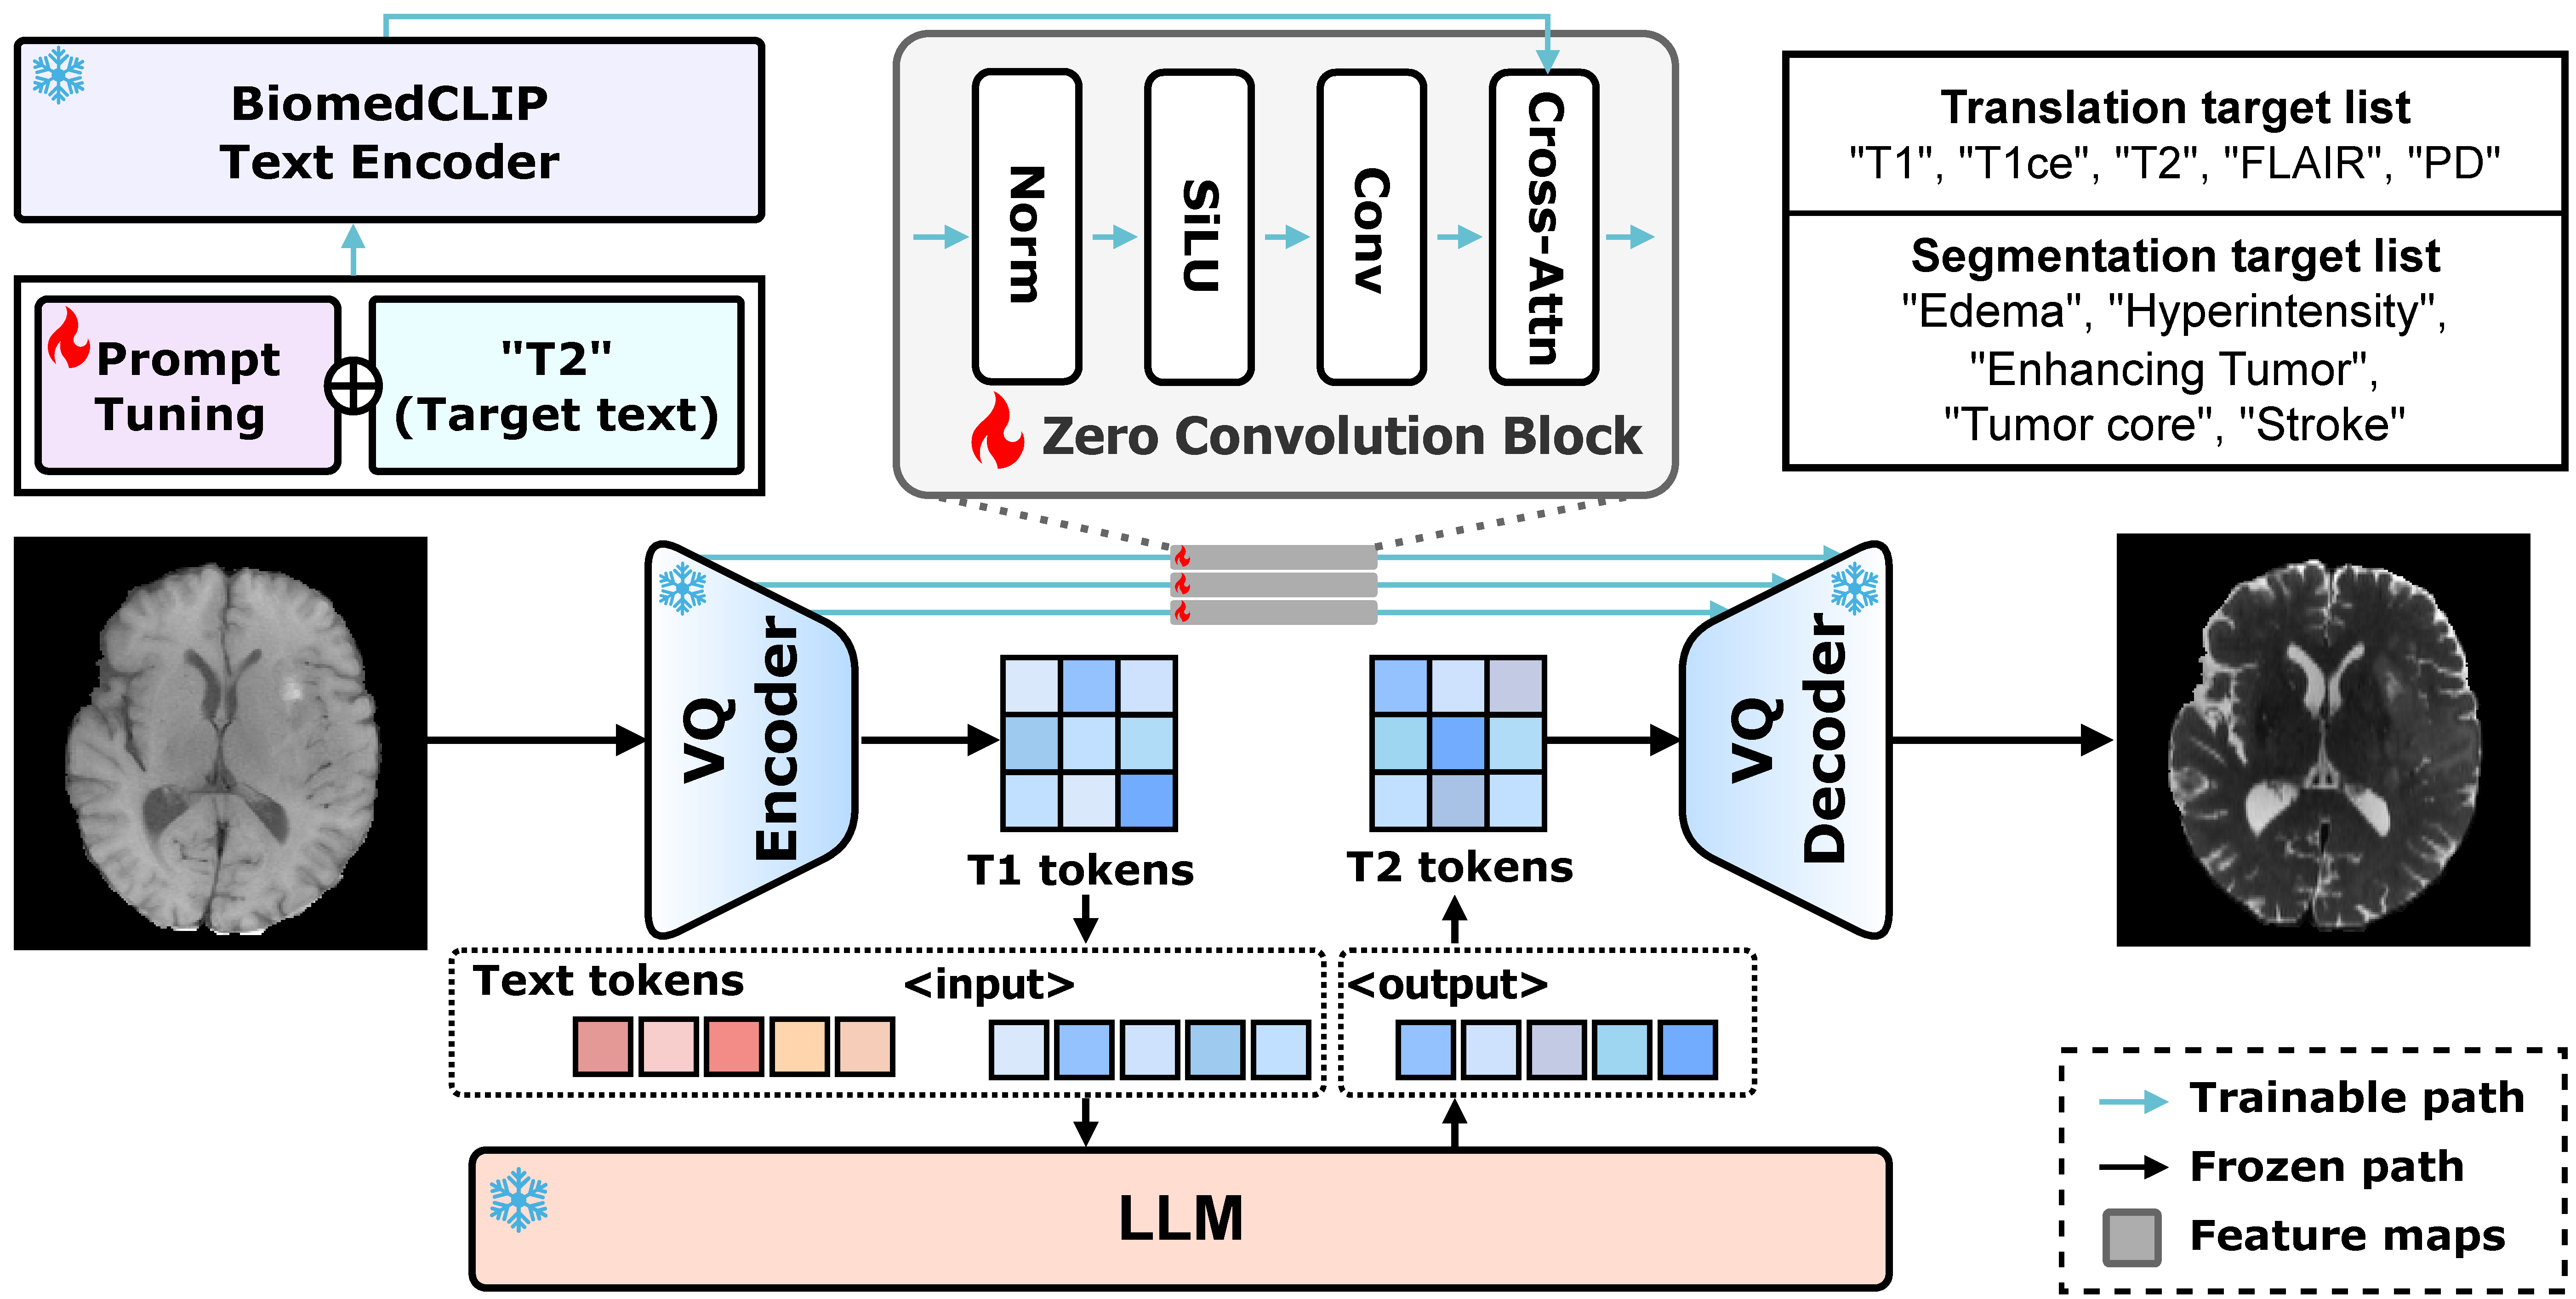
\includegraphics[width=0.85\columnwidth]{figs/fig4.pdf}
    \vspace{-3pt}
    \caption{\textbf{Fine-tuning of VQ-GAN with zero skip connection}. The skip connection is fine-tuned, while freezing the image encoder and decoder. A zero convolution block is adopted using a BiomedCLIP text encoder and prompt tuning to flexibly adapt to the target.}
    \vspace{-6pt}
    \label{fig4}
\end{figure}

\subsection{Stage II: Skip Connection Fine-tuning}
The LLM alone can perform image translation with only Stage I instruction tuning, but compressing images into latents makes it difficult to capture fine details \cite{esser2021taming,rombach2022high}. The skip connection in U-Net \cite{ronneberger2015u} preserves fine-scale information with minimal loss that works effectively in image translation. Inspired by this, we add a learnable skip connection for image translation that preserves fine-scale information (shown in Figure \ref{fig4}).

\begin{figure} [t]
    \vspace{-6pt}
    \centering
    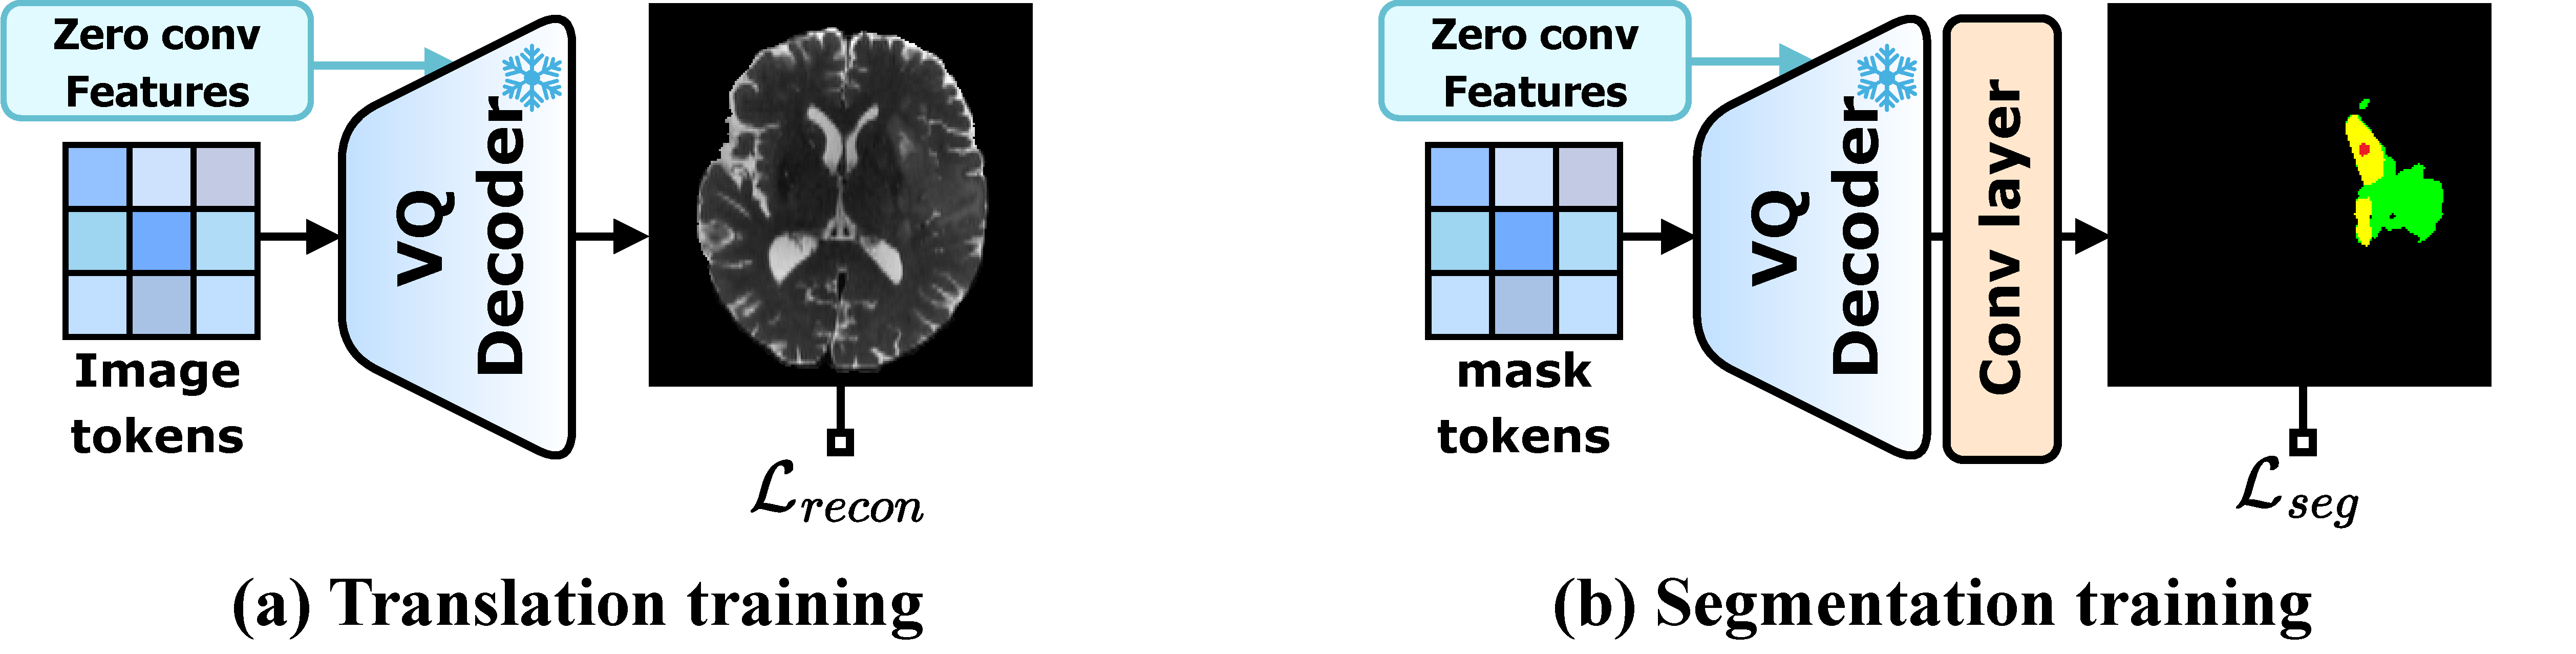
\includegraphics[width=0.9\columnwidth]{figs/fig5.pdf}
    \vspace{-3pt}
    \caption{\textbf{Loss functions for image-to-image tasks.} (a) The translation task is trained using reconstruction loss. (b) The segmentation task is trained using Dice loss with an additional layer.}
    \vspace{-6pt}
    \label{fig5}
\end{figure}

\vspace{3pt}
\noindent \textbf{Zero Convolution Block.}
Adding a skip connection initialized with random weights may disrupt the decoding process by causing significant changes in the feature map. We employ zero-initialized convolutions on each feature map, allowing them to be adapted gradually. To flexibly drive the features to the target, we incorporate a BioMedCLIP \cite{zhang2023biomedclip} text encoder along with prompt tuning \cite{jia2022visual,kim2026visual}. We define the prompt $\mathcal{P}$ as follows:
\begin{equation}
    \mathcal{P} = \text{Concat}(P(y_t),\text{CLIP}_\texttt{token}(y_t)),
\end{equation}
where $\text{Concat}$ is the concatenation operation, $P$ represents the learnable prompt, $\text{CLIP}_\texttt{token}$ is the token generated by the BioMedCLIP tokenizer, and $y_t$ is the target text. This prompt is fed into the text encoder and interacts with the image features through cross-attention. We then compute the feature of the  $i$-th skip connection as follows:
\begin{equation}
    f^\texttt{skip}_i = \text{ZeroConv}(f^\texttt{enc}_{i}, \mathcal{P}),
\end{equation}
where $f^\texttt{enc}_{i}$ denotes the $i$-th encoder feature, $\text{ZeroConv}$ represents the zero convolution block, and $f^\texttt{skip}_i$ is the resulting $i$-th skip-connection feature. The decoder feature is updated by adding the output of the $i$-th decoder layer to the corresponding skip-connection feature.

\vspace{3pt}
\noindent \textbf{Loss Function.} Since the VQ decoder produces continuous-valued images, an additional convolution layer is added to the segmentation task to generate class probabilities. We use the reconstruction loss $\mathcal{L}_{recon}$ and the segmentation loss $\mathcal{L}_{seg}$ as follows (shown in Figure \ref{fig5}):
\begin{equation}
    \mathcal{L}_{recon} = ||y-\hat{y}||^2, \ \ \mathcal{L}_{seg} = \text{DICE}(y, \hat{y}),
\end{equation}
where $y$ denotes the target and $\hat{y}$ represents the prediction.
